\subsubsection{Correzione per angolo solido finito}

Nell'analizzare la dipendenza angolare delle rate di acquisizione per verificare l'anisotropia dell'emissione del secondo gamma si è in prima trascurata la dimensione finita del rivelatore 
considerandolo puntiforme. Ovviamente tale approssimazione porta a degli errori nell'analisi dati, soprattutto per il fatto che la funzione di correlazione non è costante su tutto l'angolo solido
spazzato dal rivelatore. Al fine di correggere questa inesattezza, si può pensare di ricavare per ogni angolo $\alpha$ tra i due rivelatori un angolo $\bar\alpha$ tale che l'integrale sull'angolo
sotteso dal rivelatore posto ad un angolo $\alpha$ della funzione di correlazione sia pari all'integrale di una distribuzione uniforme sull'angolo sotteso dal rivelatore posto invece ad un angolo 
$\bar\alpha$. Prima di proseguire con il calcolo vero e proprio riduciamo le dimensioni del problema a due essendo il calcolo in 3D troppo complicato \footnote{
Si è provato a risolvere il problema 3D ma non si è giunti a risultati utilizzabili}, inoltre i suppone che
il primo fotone interagisca con il rivelatore uno esattamente al centro di quest'ultimo. Il secondo fotone sarà quindi parametrizzato da un angolo $\theta$ rispetto alla traiettoria
del primo. Definendo per comodità 
\begin{equation}
	G := \arctan{\left(\frac{r}{R}\right)}
\end{equation}
, con $ r $ raggio del rivelatore ed $ R $ distanza del rivelatore dalla sorgente, il computo da svolgere,
sapendo che la distribuzione di probabilità dell'emissione del secondo fotone in funzione dell'angolo tra i due fotoni è $1 + a \cos ^ 2 \theta + b \cos^4 \theta$,
è quindi:
\begin{equation}
	\int_{\alpha -G}^{\alpha +G} \left[ b \cos^4 \theta + a \cos ^ 2  \theta + 1 \right] \dd \theta = \left[ b \cos^4 \bar\alpha + a \cos ^ 2 \bar\alpha + 1 \right] \int_{-G}^{G} \dd\theta = \left[ b \cos^4 \bar\alpha + a \cos ^ 2 \bar \alpha + 1 \right] \left( 2G \right)
\end{equation}
Risolvendo il primo integrale si ottiene:
\begin{equation}
	\int_{\alpha -G}^{\alpha + G} \left[ b \cos^4 \theta + a \cos ^ 2  \theta + 1 \right] \dd \theta = 
\frac{b}{4}\left[ \sin \left( \alpha + G \right) \cos^3 \left( \alpha + G \right) - \sin \left( \alpha - G \right) \cos^3 \left( \alpha - G \right) \right] + \left( \frac{3b}{8} + \frac{a}{2} \right)\left[ \sin \left( \alpha + G \right) \cos \left( \alpha + G \right) - \sin \left( \alpha - G \right) \cos \left( \alpha - G \right) \right] 
+ \left( \frac{3b}{4} + a + 2 \right)G
\end{equation}
Definiamo
\begin{equation}
	I := \frac{1}{2G} \left[ \frac{b}{4}\left[ \sin \left( \alpha + G \right) \cos^3 \left( \alpha + G \right) - \sin \left( \alpha - G \right) \cos^3 \left( \alpha - G \right) \right] \right.\left. + \left( \frac{3b}{8} + \frac{a}{2} \right)\left[ \sin \left( \alpha + G \right) \cos \left( \alpha + G \right) - \sin \left( \alpha - G \right) \cos \left( \alpha - G \right) \right] + \left( \frac{3b}{4} + a + 2 \right) G \right]
\end{equation}
Dunque per ricavarsi l'angolo $ \bar \alpha $ bisogna adesso semplicemente risolvere la seguente equazione biquadratica: 
\begin{equation}
	b \cos^4 \bar\alpha + a \cos ^ 2 \bar \alpha + 1 - I= 0
\end{equation}
Tale equazione ha come soluzioni:
\begin{equation}
	\cos^2 \bar \theta  = \frac{-a + \sqrt{a^2 - 4b(1 - I)}}{2b}
	\label{fun:corr_ang}
\end{equation}
dove si è già scartata la soluzione col ``$-$''.

\begin{table}[h]
	\centering
	\begin{center}
\begin{tabulary}{\textwidth}{CCCC}
\toprule
Angoli misurati [gradi]	& Correzione per asse [gradi]	& Correzione distanza	& Correzione per finitezza [gradi]	\\ \midrule
180     & 180.452       & 1.001 & 170.895	\\ \midrule
170     & 170.459       & 0.999 & 167.005	\\ \midrule
160     & 160.451       & 0.999 & 158.921	\\ \midrule
150     & 150.43        & 0.997 & 149.841	\\ \midrule
140     & 140.396       & 0.996 & 140.446	\\ \midrule
130     & 130.35        & 0.995 & 130.938	\\ \midrule
120     & 120.293       & 0.994 & 121.433	\\ \midrule
110     & 110.226       & 0.993 & 112.121	\\ \midrule
100     & 100.153       & 0.992 & 103.648	\\ \midrule
90      & 90.075        & 0.992 & 99.1431
\end{tabulary}
\end{center}   

	\caption{Tabella delle correzioni effettuate sugli angoli considerando l'angolo solido finito sotteso dal rivelatore}
	\label{tab:fini_correzioni}
\end{table}

Per ottenere i punti da interpolare si applica la formula \ref{fun:corr_ang} ai punti già corretti per la posizione della sorgente (Tabella \ref{tab:asse_correzioni_2}) per ottenere la Tabella \ref{tab:fini_correzioni}. Dai valori in questa tabella si può arrivare al grafico di Figura \ref{gr:correl_fini}, che una volta interpolato da i parametri

$$a=0.14 \pm 0.02$$
$$b=0.0 \pm 0.1$$

che sono pienamente compatibili con quelli teorici, seppur a causa degli errori alti (14\% per a).

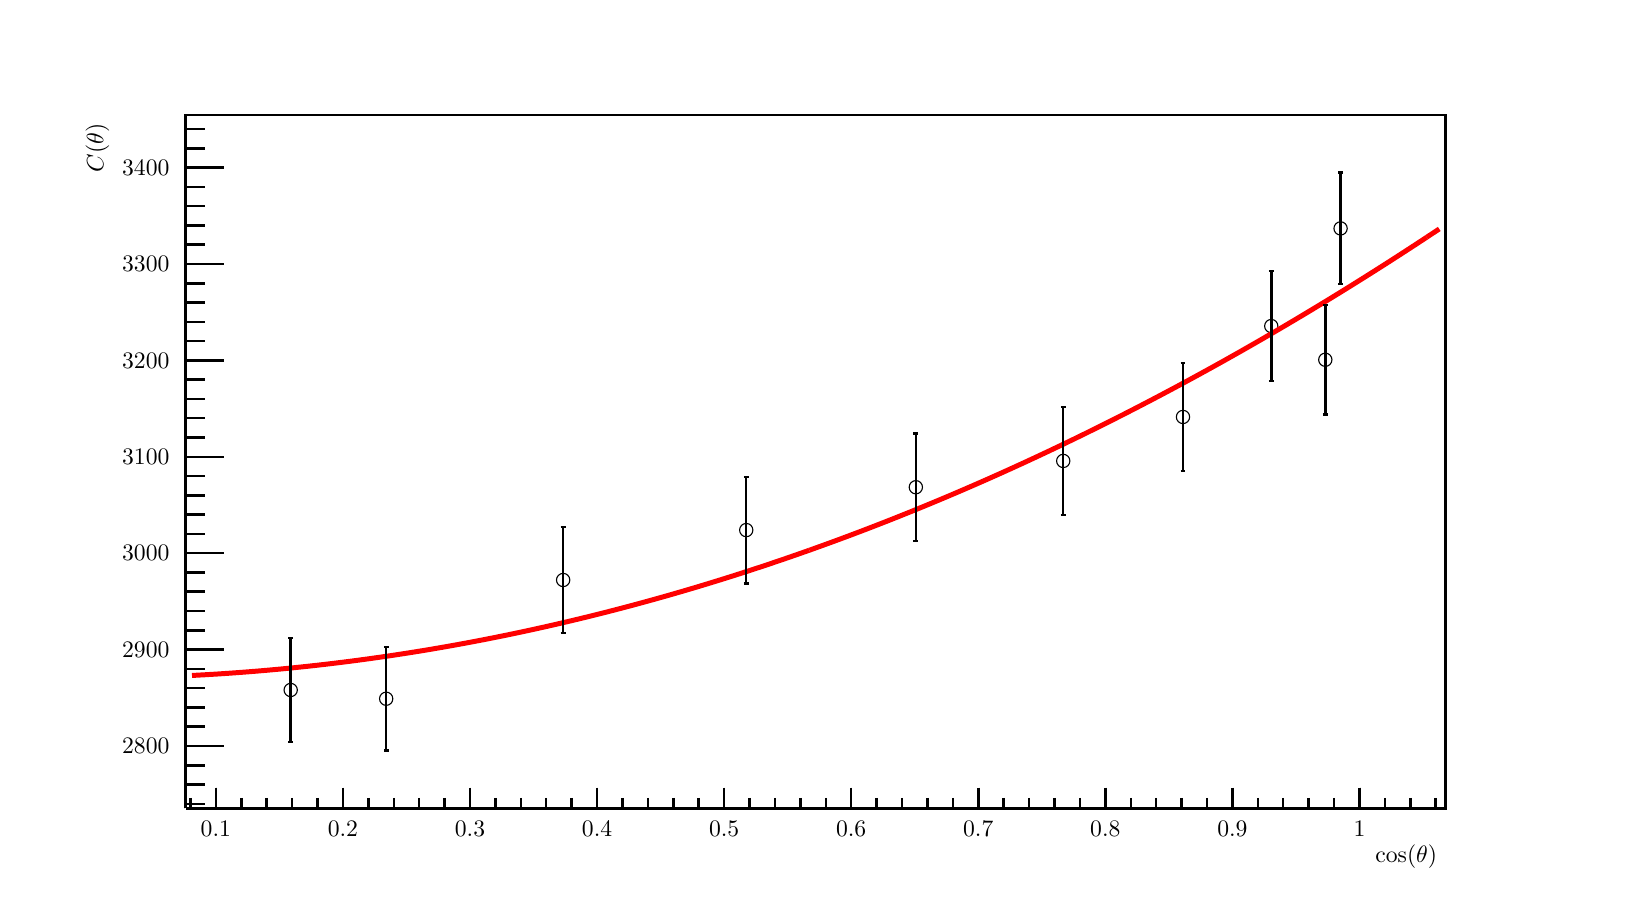
\begin{tikzpicture}
\pgfdeclareplotmark{cross} {
\pgfpathmoveto{\pgfpoint{-0.3\pgfplotmarksize}{\pgfplotmarksize}}
\pgfpathlineto{\pgfpoint{+0.3\pgfplotmarksize}{\pgfplotmarksize}}
\pgfpathlineto{\pgfpoint{+0.3\pgfplotmarksize}{0.3\pgfplotmarksize}}
\pgfpathlineto{\pgfpoint{+1\pgfplotmarksize}{0.3\pgfplotmarksize}}
\pgfpathlineto{\pgfpoint{+1\pgfplotmarksize}{-0.3\pgfplotmarksize}}
\pgfpathlineto{\pgfpoint{+0.3\pgfplotmarksize}{-0.3\pgfplotmarksize}}
\pgfpathlineto{\pgfpoint{+0.3\pgfplotmarksize}{-1.\pgfplotmarksize}}
\pgfpathlineto{\pgfpoint{-0.3\pgfplotmarksize}{-1.\pgfplotmarksize}}
\pgfpathlineto{\pgfpoint{-0.3\pgfplotmarksize}{-0.3\pgfplotmarksize}}
\pgfpathlineto{\pgfpoint{-1.\pgfplotmarksize}{-0.3\pgfplotmarksize}}
\pgfpathlineto{\pgfpoint{-1.\pgfplotmarksize}{0.3\pgfplotmarksize}}
\pgfpathlineto{\pgfpoint{-0.3\pgfplotmarksize}{0.3\pgfplotmarksize}}
\pgfpathclose
\pgfusepathqstroke
}
\pgfdeclareplotmark{cross*} {
\pgfpathmoveto{\pgfpoint{-0.3\pgfplotmarksize}{\pgfplotmarksize}}
\pgfpathlineto{\pgfpoint{+0.3\pgfplotmarksize}{\pgfplotmarksize}}
\pgfpathlineto{\pgfpoint{+0.3\pgfplotmarksize}{0.3\pgfplotmarksize}}
\pgfpathlineto{\pgfpoint{+1\pgfplotmarksize}{0.3\pgfplotmarksize}}
\pgfpathlineto{\pgfpoint{+1\pgfplotmarksize}{-0.3\pgfplotmarksize}}
\pgfpathlineto{\pgfpoint{+0.3\pgfplotmarksize}{-0.3\pgfplotmarksize}}
\pgfpathlineto{\pgfpoint{+0.3\pgfplotmarksize}{-1.\pgfplotmarksize}}
\pgfpathlineto{\pgfpoint{-0.3\pgfplotmarksize}{-1.\pgfplotmarksize}}
\pgfpathlineto{\pgfpoint{-0.3\pgfplotmarksize}{-0.3\pgfplotmarksize}}
\pgfpathlineto{\pgfpoint{-1.\pgfplotmarksize}{-0.3\pgfplotmarksize}}
\pgfpathlineto{\pgfpoint{-1.\pgfplotmarksize}{0.3\pgfplotmarksize}}
\pgfpathlineto{\pgfpoint{-0.3\pgfplotmarksize}{0.3\pgfplotmarksize}}
\pgfpathclose
\pgfusepathqfillstroke
}
\pgfdeclareplotmark{newstar} {
\pgfpathmoveto{\pgfqpoint{0pt}{\pgfplotmarksize}}
\pgfpathlineto{\pgfqpointpolar{44}{0.5\pgfplotmarksize}}
\pgfpathlineto{\pgfqpointpolar{18}{\pgfplotmarksize}}
\pgfpathlineto{\pgfqpointpolar{-20}{0.5\pgfplotmarksize}}
\pgfpathlineto{\pgfqpointpolar{-54}{\pgfplotmarksize}}
\pgfpathlineto{\pgfqpointpolar{-90}{0.5\pgfplotmarksize}}
\pgfpathlineto{\pgfqpointpolar{234}{\pgfplotmarksize}}
\pgfpathlineto{\pgfqpointpolar{198}{0.5\pgfplotmarksize}}
\pgfpathlineto{\pgfqpointpolar{162}{\pgfplotmarksize}}
\pgfpathlineto{\pgfqpointpolar{134}{0.5\pgfplotmarksize}}
\pgfpathclose
\pgfusepathqstroke
}
\pgfdeclareplotmark{newstar*} {
\pgfpathmoveto{\pgfqpoint{0pt}{\pgfplotmarksize}}
\pgfpathlineto{\pgfqpointpolar{44}{0.5\pgfplotmarksize}}
\pgfpathlineto{\pgfqpointpolar{18}{\pgfplotmarksize}}
\pgfpathlineto{\pgfqpointpolar{-20}{0.5\pgfplotmarksize}}
\pgfpathlineto{\pgfqpointpolar{-54}{\pgfplotmarksize}}
\pgfpathlineto{\pgfqpointpolar{-90}{0.5\pgfplotmarksize}}
\pgfpathlineto{\pgfqpointpolar{234}{\pgfplotmarksize}}
\pgfpathlineto{\pgfqpointpolar{198}{0.5\pgfplotmarksize}}
\pgfpathlineto{\pgfqpointpolar{162}{\pgfplotmarksize}}
\pgfpathlineto{\pgfqpointpolar{134}{0.5\pgfplotmarksize}}
\pgfpathclose
\pgfusepathqfillstroke
}
\definecolor{c}{rgb}{1,1,1};
\draw [color=c, fill=c] (0,0) rectangle (20,11.0085);
\draw [color=c, fill=c] (2,1.10085) rectangle (18,9.90762);
\definecolor{c}{rgb}{0,0,0};
\draw [c,line width=0.9] (2,1.10085) -- (2,9.90762) -- (18,9.90762) -- (18,1.10085) -- (2,1.10085);
\definecolor{c}{rgb}{1,1,1};
\draw [color=c, fill=c] (2,1.10085) rectangle (18,9.90762);
\definecolor{c}{rgb}{0,0,0};
\draw [c,line width=0.9] (2,1.10085) -- (2,9.90762) -- (18,9.90762) -- (18,1.10085) -- (2,1.10085);
\draw [c,line width=0.9] (2,1.10085) -- (18,1.10085);
\draw [anchor= east] (18,0.484373) node[scale=0.854877, color=c, rotate=0]{$\cos(\theta)$};
\draw [c,line width=0.9] (2.3829,1.36505) -- (2.3829,1.10085);
\draw [c,line width=0.9] (2.70565,1.23295) -- (2.70565,1.10085);
\draw [c,line width=0.9] (3.0284,1.23295) -- (3.0284,1.10085);
\draw [c,line width=0.9] (3.35116,1.23295) -- (3.35116,1.10085);
\draw [c,line width=0.9] (3.67391,1.23295) -- (3.67391,1.10085);
\draw [c,line width=0.9] (3.99666,1.36505) -- (3.99666,1.10085);
\draw [c,line width=0.9] (4.31941,1.23295) -- (4.31941,1.10085);
\draw [c,line width=0.9] (4.64216,1.23295) -- (4.64216,1.10085);
\draw [c,line width=0.9] (4.96491,1.23295) -- (4.96491,1.10085);
\draw [c,line width=0.9] (5.28766,1.23295) -- (5.28766,1.10085);
\draw [c,line width=0.9] (5.61041,1.36505) -- (5.61041,1.10085);
\draw [c,line width=0.9] (5.93316,1.23295) -- (5.93316,1.10085);
\draw [c,line width=0.9] (6.25591,1.23295) -- (6.25591,1.10085);
\draw [c,line width=0.9] (6.57866,1.23295) -- (6.57866,1.10085);
\draw [c,line width=0.9] (6.90141,1.23295) -- (6.90141,1.10085);
\draw [c,line width=0.9] (7.22416,1.36505) -- (7.22416,1.10085);
\draw [c,line width=0.9] (7.54691,1.23295) -- (7.54691,1.10085);
\draw [c,line width=0.9] (7.86966,1.23295) -- (7.86966,1.10085);
\draw [c,line width=0.9] (8.19241,1.23295) -- (8.19241,1.10085);
\draw [c,line width=0.9] (8.51516,1.23295) -- (8.51516,1.10085);
\draw [c,line width=0.9] (8.83791,1.36505) -- (8.83791,1.10085);
\draw [c,line width=0.9] (9.16066,1.23295) -- (9.16066,1.10085);
\draw [c,line width=0.9] (9.48341,1.23295) -- (9.48341,1.10085);
\draw [c,line width=0.9] (9.80616,1.23295) -- (9.80616,1.10085);
\draw [c,line width=0.9] (10.1289,1.23295) -- (10.1289,1.10085);
\draw [c,line width=0.9] (10.4517,1.36505) -- (10.4517,1.10085);
\draw [c,line width=0.9] (10.7744,1.23295) -- (10.7744,1.10085);
\draw [c,line width=0.9] (11.0972,1.23295) -- (11.0972,1.10085);
\draw [c,line width=0.9] (11.4199,1.23295) -- (11.4199,1.10085);
\draw [c,line width=0.9] (11.7427,1.23295) -- (11.7427,1.10085);
\draw [c,line width=0.9] (12.0654,1.36505) -- (12.0654,1.10085);
\draw [c,line width=0.9] (12.3882,1.23295) -- (12.3882,1.10085);
\draw [c,line width=0.9] (12.7109,1.23295) -- (12.7109,1.10085);
\draw [c,line width=0.9] (13.0337,1.23295) -- (13.0337,1.10085);
\draw [c,line width=0.9] (13.3564,1.23295) -- (13.3564,1.10085);
\draw [c,line width=0.9] (13.6792,1.36505) -- (13.6792,1.10085);
\draw [c,line width=0.9] (14.0019,1.23295) -- (14.0019,1.10085);
\draw [c,line width=0.9] (14.3247,1.23295) -- (14.3247,1.10085);
\draw [c,line width=0.9] (14.6474,1.23295) -- (14.6474,1.10085);
\draw [c,line width=0.9] (14.9702,1.23295) -- (14.9702,1.10085);
\draw [c,line width=0.9] (15.2929,1.36505) -- (15.2929,1.10085);
\draw [c,line width=0.9] (15.6157,1.23295) -- (15.6157,1.10085);
\draw [c,line width=0.9] (15.9384,1.23295) -- (15.9384,1.10085);
\draw [c,line width=0.9] (16.2612,1.23295) -- (16.2612,1.10085);
\draw [c,line width=0.9] (16.5839,1.23295) -- (16.5839,1.10085);
\draw [c,line width=0.9] (16.9067,1.36505) -- (16.9067,1.10085);
\draw [c,line width=0.9] (2.3829,1.36505) -- (2.3829,1.10085);
\draw [c,line width=0.9] (2.06015,1.23295) -- (2.06015,1.10085);
\draw [c,line width=0.9] (16.9067,1.36505) -- (16.9067,1.10085);
\draw [c,line width=0.9] (17.2294,1.23295) -- (17.2294,1.10085);
\draw [c,line width=0.9] (17.5522,1.23295) -- (17.5522,1.10085);
\draw [c,line width=0.9] (17.8749,1.23295) -- (17.8749,1.10085);
\draw [anchor=base] (2.3829,0.737567) node[scale=0.854877, color=c, rotate=0]{0.1};
\draw [anchor=base] (3.99666,0.737567) node[scale=0.854877, color=c, rotate=0]{0.2};
\draw [anchor=base] (5.61041,0.737567) node[scale=0.854877, color=c, rotate=0]{0.3};
\draw [anchor=base] (7.22416,0.737567) node[scale=0.854877, color=c, rotate=0]{0.4};
\draw [anchor=base] (8.83791,0.737567) node[scale=0.854877, color=c, rotate=0]{0.5};
\draw [anchor=base] (10.4517,0.737567) node[scale=0.854877, color=c, rotate=0]{0.6};
\draw [anchor=base] (12.0654,0.737567) node[scale=0.854877, color=c, rotate=0]{0.7};
\draw [anchor=base] (13.6792,0.737567) node[scale=0.854877, color=c, rotate=0]{0.8};
\draw [anchor=base] (15.2929,0.737567) node[scale=0.854877, color=c, rotate=0]{0.9};
\draw [anchor=base] (16.9067,0.737567) node[scale=0.854877, color=c, rotate=0]{1};
\draw [c,line width=0.9] (2,1.10085) -- (2,9.90762);
\draw [anchor= east] (0.88,9.90762) node[scale=0.854877, color=c, rotate=90]{$C(\theta)$};
\draw [c,line width=0.9] (2.48,1.89304) -- (2,1.89304);
\draw [c,line width=0.9] (2.24,2.13789) -- (2,2.13789);
\draw [c,line width=0.9] (2.24,2.38273) -- (2,2.38273);
\draw [c,line width=0.9] (2.24,2.62758) -- (2,2.62758);
\draw [c,line width=0.9] (2.24,2.87242) -- (2,2.87242);
\draw [c,line width=0.9] (2.48,3.11727) -- (2,3.11727);
\draw [c,line width=0.9] (2.24,3.36211) -- (2,3.36211);
\draw [c,line width=0.9] (2.24,3.60696) -- (2,3.60696);
\draw [c,line width=0.9] (2.24,3.85181) -- (2,3.85181);
\draw [c,line width=0.9] (2.24,4.09665) -- (2,4.09665);
\draw [c,line width=0.9] (2.48,4.3415) -- (2,4.3415);
\draw [c,line width=0.9] (2.24,4.58634) -- (2,4.58634);
\draw [c,line width=0.9] (2.24,4.83119) -- (2,4.83119);
\draw [c,line width=0.9] (2.24,5.07603) -- (2,5.07603);
\draw [c,line width=0.9] (2.24,5.32088) -- (2,5.32088);
\draw [c,line width=0.9] (2.48,5.56572) -- (2,5.56572);
\draw [c,line width=0.9] (2.24,5.81057) -- (2,5.81057);
\draw [c,line width=0.9] (2.24,6.05542) -- (2,6.05542);
\draw [c,line width=0.9] (2.24,6.30026) -- (2,6.30026);
\draw [c,line width=0.9] (2.24,6.54511) -- (2,6.54511);
\draw [c,line width=0.9] (2.48,6.78995) -- (2,6.78995);
\draw [c,line width=0.9] (2.24,7.0348) -- (2,7.0348);
\draw [c,line width=0.9] (2.24,7.27964) -- (2,7.27964);
\draw [c,line width=0.9] (2.24,7.52449) -- (2,7.52449);
\draw [c,line width=0.9] (2.24,7.76933) -- (2,7.76933);
\draw [c,line width=0.9] (2.48,8.01418) -- (2,8.01418);
\draw [c,line width=0.9] (2.24,8.25902) -- (2,8.25902);
\draw [c,line width=0.9] (2.24,8.50387) -- (2,8.50387);
\draw [c,line width=0.9] (2.24,8.74872) -- (2,8.74872);
\draw [c,line width=0.9] (2.24,8.99356) -- (2,8.99356);
\draw [c,line width=0.9] (2.48,9.23841) -- (2,9.23841);
\draw [c,line width=0.9] (2.48,1.89304) -- (2,1.89304);
\draw [c,line width=0.9] (2.24,1.6482) -- (2,1.6482);
\draw [c,line width=0.9] (2.24,1.40335) -- (2,1.40335);
\draw [c,line width=0.9] (2.24,1.15851) -- (2,1.15851);
\draw [c,line width=0.9] (2.48,9.23841) -- (2,9.23841);
\draw [c,line width=0.9] (2.24,9.48325) -- (2,9.48325);
\draw [c,line width=0.9] (2.24,9.7281) -- (2,9.7281);
\draw [anchor= east] (1.9,1.89304) node[scale=0.854877, color=c, rotate=0]{2800};
\draw [anchor= east] (1.9,3.11727) node[scale=0.854877, color=c, rotate=0]{2900};
\draw [anchor= east] (1.9,4.3415) node[scale=0.854877, color=c, rotate=0]{3000};
\draw [anchor= east] (1.9,5.56572) node[scale=0.854877, color=c, rotate=0]{3100};
\draw [anchor= east] (1.9,6.78995) node[scale=0.854877, color=c, rotate=0]{3200};
\draw [anchor= east] (1.9,8.01418) node[scale=0.854877, color=c, rotate=0]{3300};
\draw [anchor= east] (1.9,9.23841) node[scale=0.854877, color=c, rotate=0]{3400};
\foreach \P in {(16.6667,8.46612), (16.4727,6.79804), (15.7864,7.22579), (14.6654,6.07138), (13.1444,5.51302), (11.2725,5.17927), (9.1187,4.6349), (6.79348,4.00096), (4.54597,2.49294), (3.33333,2.60415)}{\draw[mark options={color=c,fill=c},mark
 size=2.402402pt,mark=o] plot coordinates {\P};}
\definecolor{c}{rgb}{1,0,0};
\draw [c,line width=1.8] (2.08,2.78861) -- (2.24,2.79724) -- (2.4,2.80686) -- (2.56,2.81748) -- (2.72,2.82909) -- (2.88,2.84169) -- (3.04,2.85529) -- (3.2,2.86987) -- (3.36,2.88545) -- (3.52,2.90203) -- (3.68,2.91959) -- (3.84,2.93815) -- (4,2.9577)
 -- (4.16,2.97825) -- (4.32,2.99979) -- (4.48,3.02232) -- (4.64,3.04584) -- (4.8,3.07036) -- (4.96,3.09587) -- (5.12,3.12237) -- (5.28,3.14986) -- (5.44,3.17835) -- (5.6,3.20783) -- (5.76,3.23831) -- (5.92,3.26977) -- (6.08,3.30223) -- (6.24,3.33568)
 -- (6.4,3.37013) -- (6.56,3.40557) -- (6.72,3.442) -- (6.88,3.47942) -- (7.04,3.51783) -- (7.2,3.55724) -- (7.36,3.59765) -- (7.52,3.63904) -- (7.68,3.68143) -- (7.84,3.72481) -- (8,3.76918) -- (8.16,3.81455) -- (8.32,3.86091) -- (8.48,3.90826) --
 (8.64,3.9566) -- (8.8,4.00594) -- (8.96,4.05627) -- (9.12,4.10759) -- (9.28,4.15991) -- (9.44,4.21322) -- (9.6,4.26752) -- (9.76,4.32282) -- (9.92,4.3791);
\draw [c,line width=1.8] (9.92,4.3791) -- (10.08,4.43638) -- (10.24,4.49466) -- (10.4,4.55392) -- (10.56,4.61418) -- (10.72,4.67543) -- (10.88,4.73768) -- (11.04,4.80092) -- (11.2,4.86515) -- (11.36,4.93037) -- (11.52,4.99659) -- (11.68,5.06379) --
 (11.84,5.132) -- (12,5.20119) -- (12.16,5.27138) -- (12.32,5.34256) -- (12.48,5.41473) -- (12.64,5.4879) -- (12.8,5.56206) -- (12.96,5.63721) -- (13.12,5.71335) -- (13.28,5.79049) -- (13.44,5.86862) -- (13.6,5.94774) -- (13.76,6.02786) --
 (13.92,6.10897) -- (14.08,6.19107) -- (14.24,6.27416) -- (14.4,6.35825) -- (14.56,6.44333) -- (14.72,6.5294) -- (14.88,6.61647) -- (15.04,6.70453) -- (15.2,6.79358) -- (15.36,6.88363) -- (15.52,6.97466) -- (15.68,7.06669) -- (15.84,7.15972) --
 (16,7.25373) -- (16.16,7.34874) -- (16.32,7.44474) -- (16.48,7.54174) -- (16.64,7.63972) -- (16.8,7.7387) -- (16.96,7.83868) -- (17.12,7.93964) -- (17.28,8.0416) -- (17.44,8.14455) -- (17.6,8.2485) -- (17.76,8.35343);
\draw [c,line width=1.8] (17.76,8.35343) -- (17.92,8.45936);
\definecolor{c}{rgb}{0,0,0};
\draw [c,line width=0.9] (16.6667,8.46612) -- (16.6667,9.17372);
\draw [c,line width=0.9] (16.6359,9.17372) -- (16.6975,9.17372);
\draw [c,line width=0.9] (16.6667,8.46612) -- (16.6667,7.75852);
\draw [c,line width=0.9] (16.6359,7.75852) -- (16.6975,7.75852);
\draw [c,line width=0.9] (16.4727,6.79804) -- (16.4727,7.49136);
\draw [c,line width=0.9] (16.442,7.49136) -- (16.5035,7.49136);
\draw [c,line width=0.9] (16.4727,6.79804) -- (16.4727,6.10471);
\draw [c,line width=0.9] (16.442,6.10471) -- (16.5035,6.10471);
\draw [c,line width=0.9] (15.7864,7.22579) -- (15.7864,7.92363);
\draw [c,line width=0.9] (15.7556,7.92363) -- (15.8172,7.92363);
\draw [c,line width=0.9] (15.7864,7.22579) -- (15.7864,6.52795);
\draw [c,line width=0.9] (15.7556,6.52795) -- (15.8172,6.52795);
\draw [c,line width=0.9] (14.6654,6.07138) -- (14.6654,6.75975);
\draw [c,line width=0.9] (14.6346,6.75975) -- (14.6962,6.75975);
\draw [c,line width=0.9] (14.6654,6.07138) -- (14.6654,5.383);
\draw [c,line width=0.9] (14.6346,5.383) -- (14.6962,5.383);
\draw [c,line width=0.9] (13.1444,5.51302) -- (13.1444,6.19713);
\draw [c,line width=0.9] (13.1136,6.19713) -- (13.1752,6.19713);
\draw [c,line width=0.9] (13.1444,5.51302) -- (13.1444,4.82892);
\draw [c,line width=0.9] (13.1136,4.82892) -- (13.1752,4.82892);
\draw [c,line width=0.9] (11.2725,5.17927) -- (11.2725,5.86103);
\draw [c,line width=0.9] (11.2417,5.86103) -- (11.3033,5.86103);
\draw [c,line width=0.9] (11.2725,5.17927) -- (11.2725,4.49752);
\draw [c,line width=0.9] (11.2417,4.49752) -- (11.3033,4.49752);
\draw [c,line width=0.9] (9.1187,4.6349) -- (9.1187,5.31226);
\draw [c,line width=0.9] (9.08791,5.31226) -- (9.1495,5.31226);
\draw [c,line width=0.9] (9.1187,4.6349) -- (9.1187,3.95753);
\draw [c,line width=0.9] (9.08791,3.95753) -- (9.1495,3.95753);
\draw [c,line width=0.9] (6.79348,4.00096) -- (6.79348,4.67294);
\draw [c,line width=0.9] (6.76268,4.67294) -- (6.82427,4.67294);
\draw [c,line width=0.9] (6.79348,4.00096) -- (6.79348,3.32899);
\draw [c,line width=0.9] (6.76268,3.32899) -- (6.82427,3.32899);
\draw [c,line width=0.9] (4.54597,2.49294) -- (4.54597,3.15114);
\draw [c,line width=0.9] (4.51517,3.15114) -- (4.57676,3.15114);
\draw [c,line width=0.9] (4.54597,2.49294) -- (4.54597,1.83474);
\draw [c,line width=0.9] (4.51517,1.83474) -- (4.57676,1.83474);
\draw [c,line width=0.9] (3.33333,2.60415) -- (3.33333,3.26351);
\draw [c,line width=0.9] (3.30254,3.26351) -- (3.36413,3.26351);
\draw [c,line width=0.9] (3.33333,2.60415) -- (3.33333,1.94479);
\draw [c,line width=0.9] (3.30254,1.94479) -- (3.36413,1.94479);
\end{tikzpicture}




